\section{Conception conjointe Matérielle/Logicielle}
La conception conjointe , est aussi appelée "codesign" qui correspond à une fonctionnalité complexe qui allie une partie logique programmée (flexibilité) et une logique câblée (performances). Utilisée pour réaliser des système complexes sur Silicium ou SOPC, dans notre cas (System On Programmable Chip) sur FPGA. Ce qui permet d'intégrer les périphériques ainsi que le processeur dans le FPGA, dans notre projet il s'agît de la réalisation d'un micrô-contrôleur.\newline

Dans le système réalisé pour le projet nous avons généré, à l'aide de "SOPC Builder", un système SOPC comportant l'ensemble des fonctions du projet à partir de leurs fichiers VHDL. Dans le système on y retrouve le processeur NIOS II sur 32 Bits qui va permettre l'exécution des fonctions codées dans la partie logicielle, de la mémoire (type SRAM) de 20 Ko, un JTAG qui va permettre de créer une interface entre l'environnement de programmation (NIOS II) et le SOPC. Pour finir un composant "SYSID" qui va permettre l'identification du système et va protéger le système de tous mauvais téléchargements de programmes ne correspondant pas à l'application.\vspace{0.5cm}
\begin{figure}[h]
    \begin{center}
      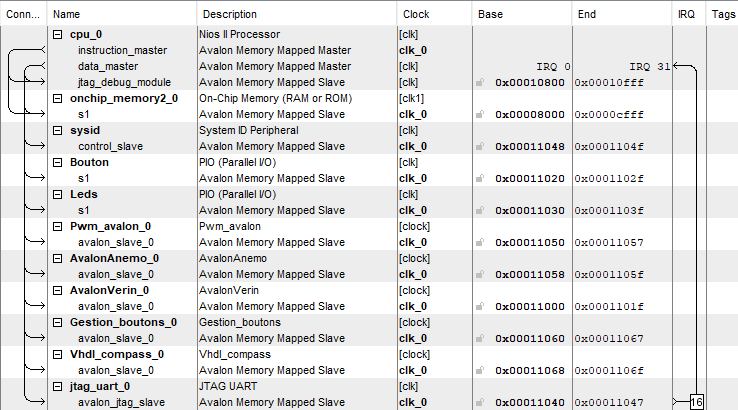
\includegraphics[width=\textwidth]{images/SOPC.png}
      \caption{Les différents composants du SOPC}
    \end{center}
  \end{figure}

  \newpage 

  Une fois les différents composants ajoutés avec leurs différents fichiers VHDL, une boite globale du projet est créée par "SOPC Builder".
\vspace{0.5cm}
  \begin{figure}[h]
    \begin{center}
      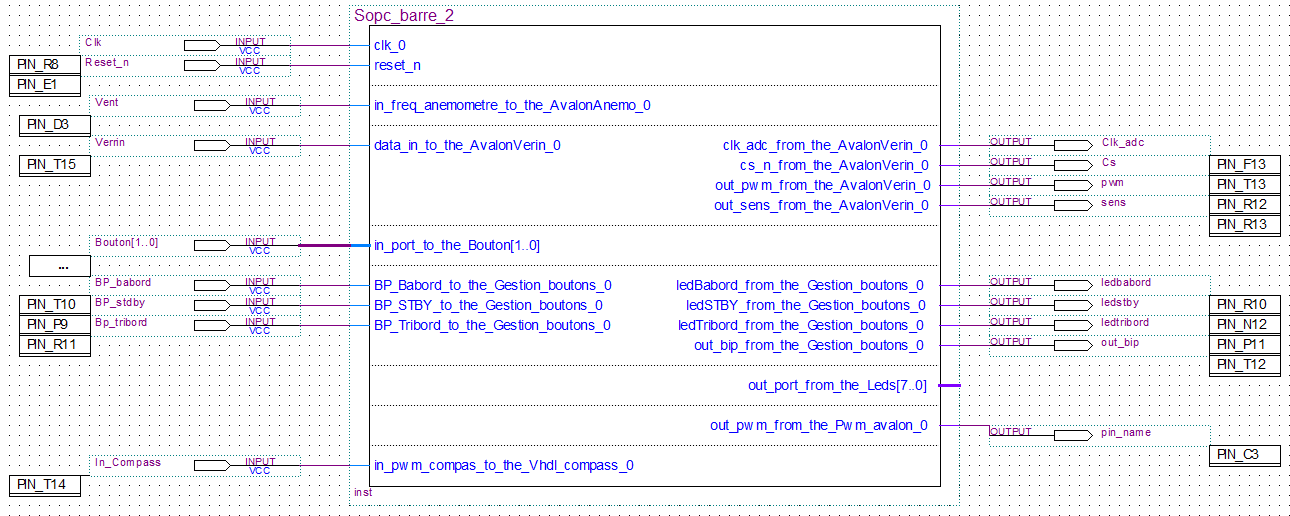
\includegraphics[width=\textwidth]{images/sopc_bloc.png}
      \caption{SOPC et ses différents ports GPIO}
    \end{center}
  \end{figure}

  Il est nécessaire, une fois la fonction de Sopc réalisée, de gérer l'affectation des pins du FPGA avec celle générées dans notre fichier sopc. Il est important de respecter les pins déjà attribuées dans le cahier des charges car certaines sont déjà câblées sur la maquette de développement.